\documentclass[12pt, letterpaper]{scrartcl}

\usepackage{fullpage} % Set margins and place page numbers at bottom center
\usepackage[shortlabels]{enumitem} % Use a. in the enumerate
\usepackage{amsmath} % aligned equations
\usepackage{graphicx} % include figure
\usepackage{float} % usage of H for figure float
\usepackage{amssymb} % \varnothing
\usepackage{subfigure}

\begin{document}

% ### Header - start ###
    \begin{center}
    	\hrule
    	\vspace{0.4cm}
    	{\textbf { {\large Homework 2} \\ EE 513 --- Stochastic Systems Theory}}
    \end{center}
    { \textbf{Name:} Ali Zafari \hspace{\fill} \textbf{Student Number:} 800350381 \hspace{\fill} \textbf{Fall 2022} } \newline\hrule
% ### Header - end ###


\paragraph*{Problem 2.1} \hfill\\
\begin{enumerate}[((a))]
    \item 
    \begin{align*}
        p_b&: \text{Probability of Board working}\\
        p&: \text{Probability of Chip working}
    \end{align*}
    \begin{flalign*}
        p_b&=P(\text{at least 7 chips out of 8 chips working})\\
        &=\binom{8}{7}p^7(1-p)+\binom{8}{8}p^8\\
        &=-8p^8+8p^7+p^8\\
        &=8p^7-7p^8
    \end{flalign*}
    
    \item 
    \begin{flalign*}
        P(\text{At least ONE board working})&\geq99.9\%\\
        1-\binom{n}{0}p_b^0(1-p_b)^n&\geq0.999\\
        0.001&\geq(1-p_b)^n\\
        -3&\geq n\log(1-p_b)\\
        \frac{-3}{\log(1-p_b)}&\leq n\\
        \frac{-3}{\log(1-8p^7-7p^8)}&\leq n
    \end{flalign*}

\end{enumerate}
\hrule
\clearpage
\paragraph*{Problem 2.2} \hfill\\
\begin{enumerate}[((a))]
    \item Area under the Laplacian pdf must be one:
    \begin{align*}
        \int^{+\infty}_{-\infty}f_X(x)dx&=1\\
        \int^{+\infty}_{-\infty}ae^{-b|x|}dx&=1\\
        a[\quad\int^{0}_{-\infty}e^{bx}dx+\int^{+\infty}_{0}e^{-bx}dx\quad]&=1\\
        a[\quad\frac{1}{b}e^{bx}\bigg\rvert^{0}_{-\infty}\quad+\quad\frac{1}{-b}e^{-bx}\bigg\rvert^{+\infty}_{0}\quad]&=1\qquad[\text{only if }b\geq0]\\
        a[\quad\frac{1}{b}(1-0)\quad+\quad\frac{1}{-b}(0-1)\quad]&=1\\
        \frac{2a}{b}&=1\\
        b&=2a
    \end{align*}
    if $a=\frac{1}{2}$ then $b=1$, then the cdf will be:
    \begin{align*}
        F_X(x)&=\int_{-\infty}^{x}\frac{1}{2}e^{-|t|}dt\\\\
        &=
        \begin{cases}
         \frac{1}{2}e^{t}\bigg\rvert^{x}_{-\infty}=\frac{1}{2}e^{x} & \qquad ,\quad x\leq 0\\\\ 
         \frac{1}{2}e^{t}\bigg\rvert^{0}_{-\infty}+\frac{-1}{2}e^{-t}\bigg\rvert^{0}_{x}=1-\frac{1}{2}e^{-x} & \qquad ,\quad x > 0
        \end{cases}\\\\
        &=
        \begin{cases}
         \frac{1}{2}e^{x} & \qquad ,\quad x\leq 0\\
         1-\frac{1}{2}e^{-x} & \qquad ,\quad x > 0
        \end{cases}
    \end{align*}
    \begin{figure}[H]
        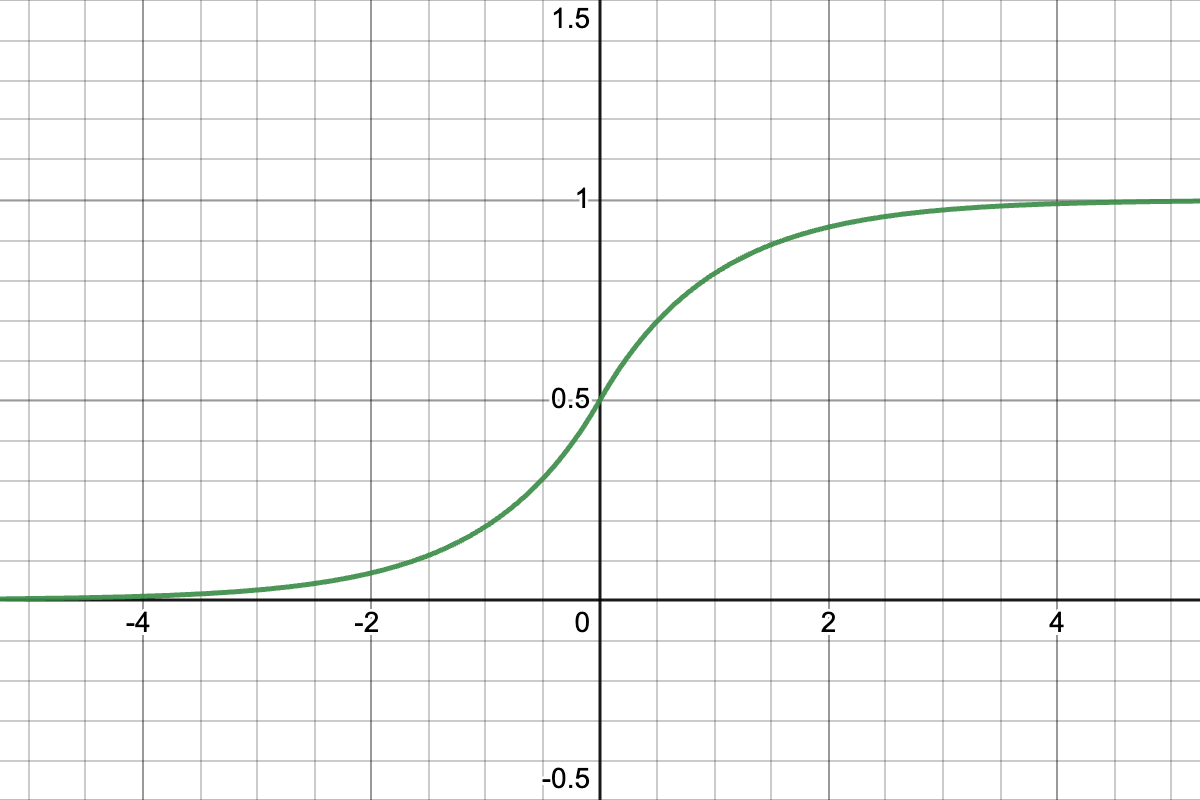
\includegraphics[width=0.7\linewidth]{hw2_figures/2.2a.png}
        \centering
        \caption{CDF $F_X(x)$}
    \end{figure}
    \item To find relationship between a and b:
    \begin{align*}
        \int^{+\infty}_{-\infty}f_X(x)dx&=1\\
        \int^{+\infty}_{-\infty}\frac{a}{b^2+x^2}&=1\\
        \frac{a}{b}\int^{+\infty}_{-\infty}\frac{\frac{1}{b}}{1+(\frac{x}{b})^2}&=1\\
        \frac{a}{b}\arctan(\frac{x}{b})\bigg\rvert^{+\infty}_{-\infty}&=1\\
        \frac{a}{b}(+\frac{\pi}{2}-(-\frac{\pi}{2}))&=1\\
        \frac{a}{b}\pi&=1\\
        b&=\pi a
    \end{align*}
    if $a=\frac{1}{2}$ then $b=\pi$, then the cdf will be:
    \begin{align*}
        F_X(x)&=\int_{-\infty}^{x}\frac{1/2}{(\frac{\pi}{2})^2+t^2}dt\\
        &=\frac{1}{\pi}\int_{-\infty}^{x}\frac{\frac{1}{\pi/2}}{1+(\frac{t}{\pi/2})^2}dt\\
        &=\frac{1}{\pi}\arctan(\frac{x}{\pi}/2)\bigg\rvert^{x}_{-\infty}\\
        &=\frac{1}{\pi}[\arctan(\frac{x}{\pi/2})+\frac{\pi}{2}]
    \end{align*}
    \begin{figure}[H]
        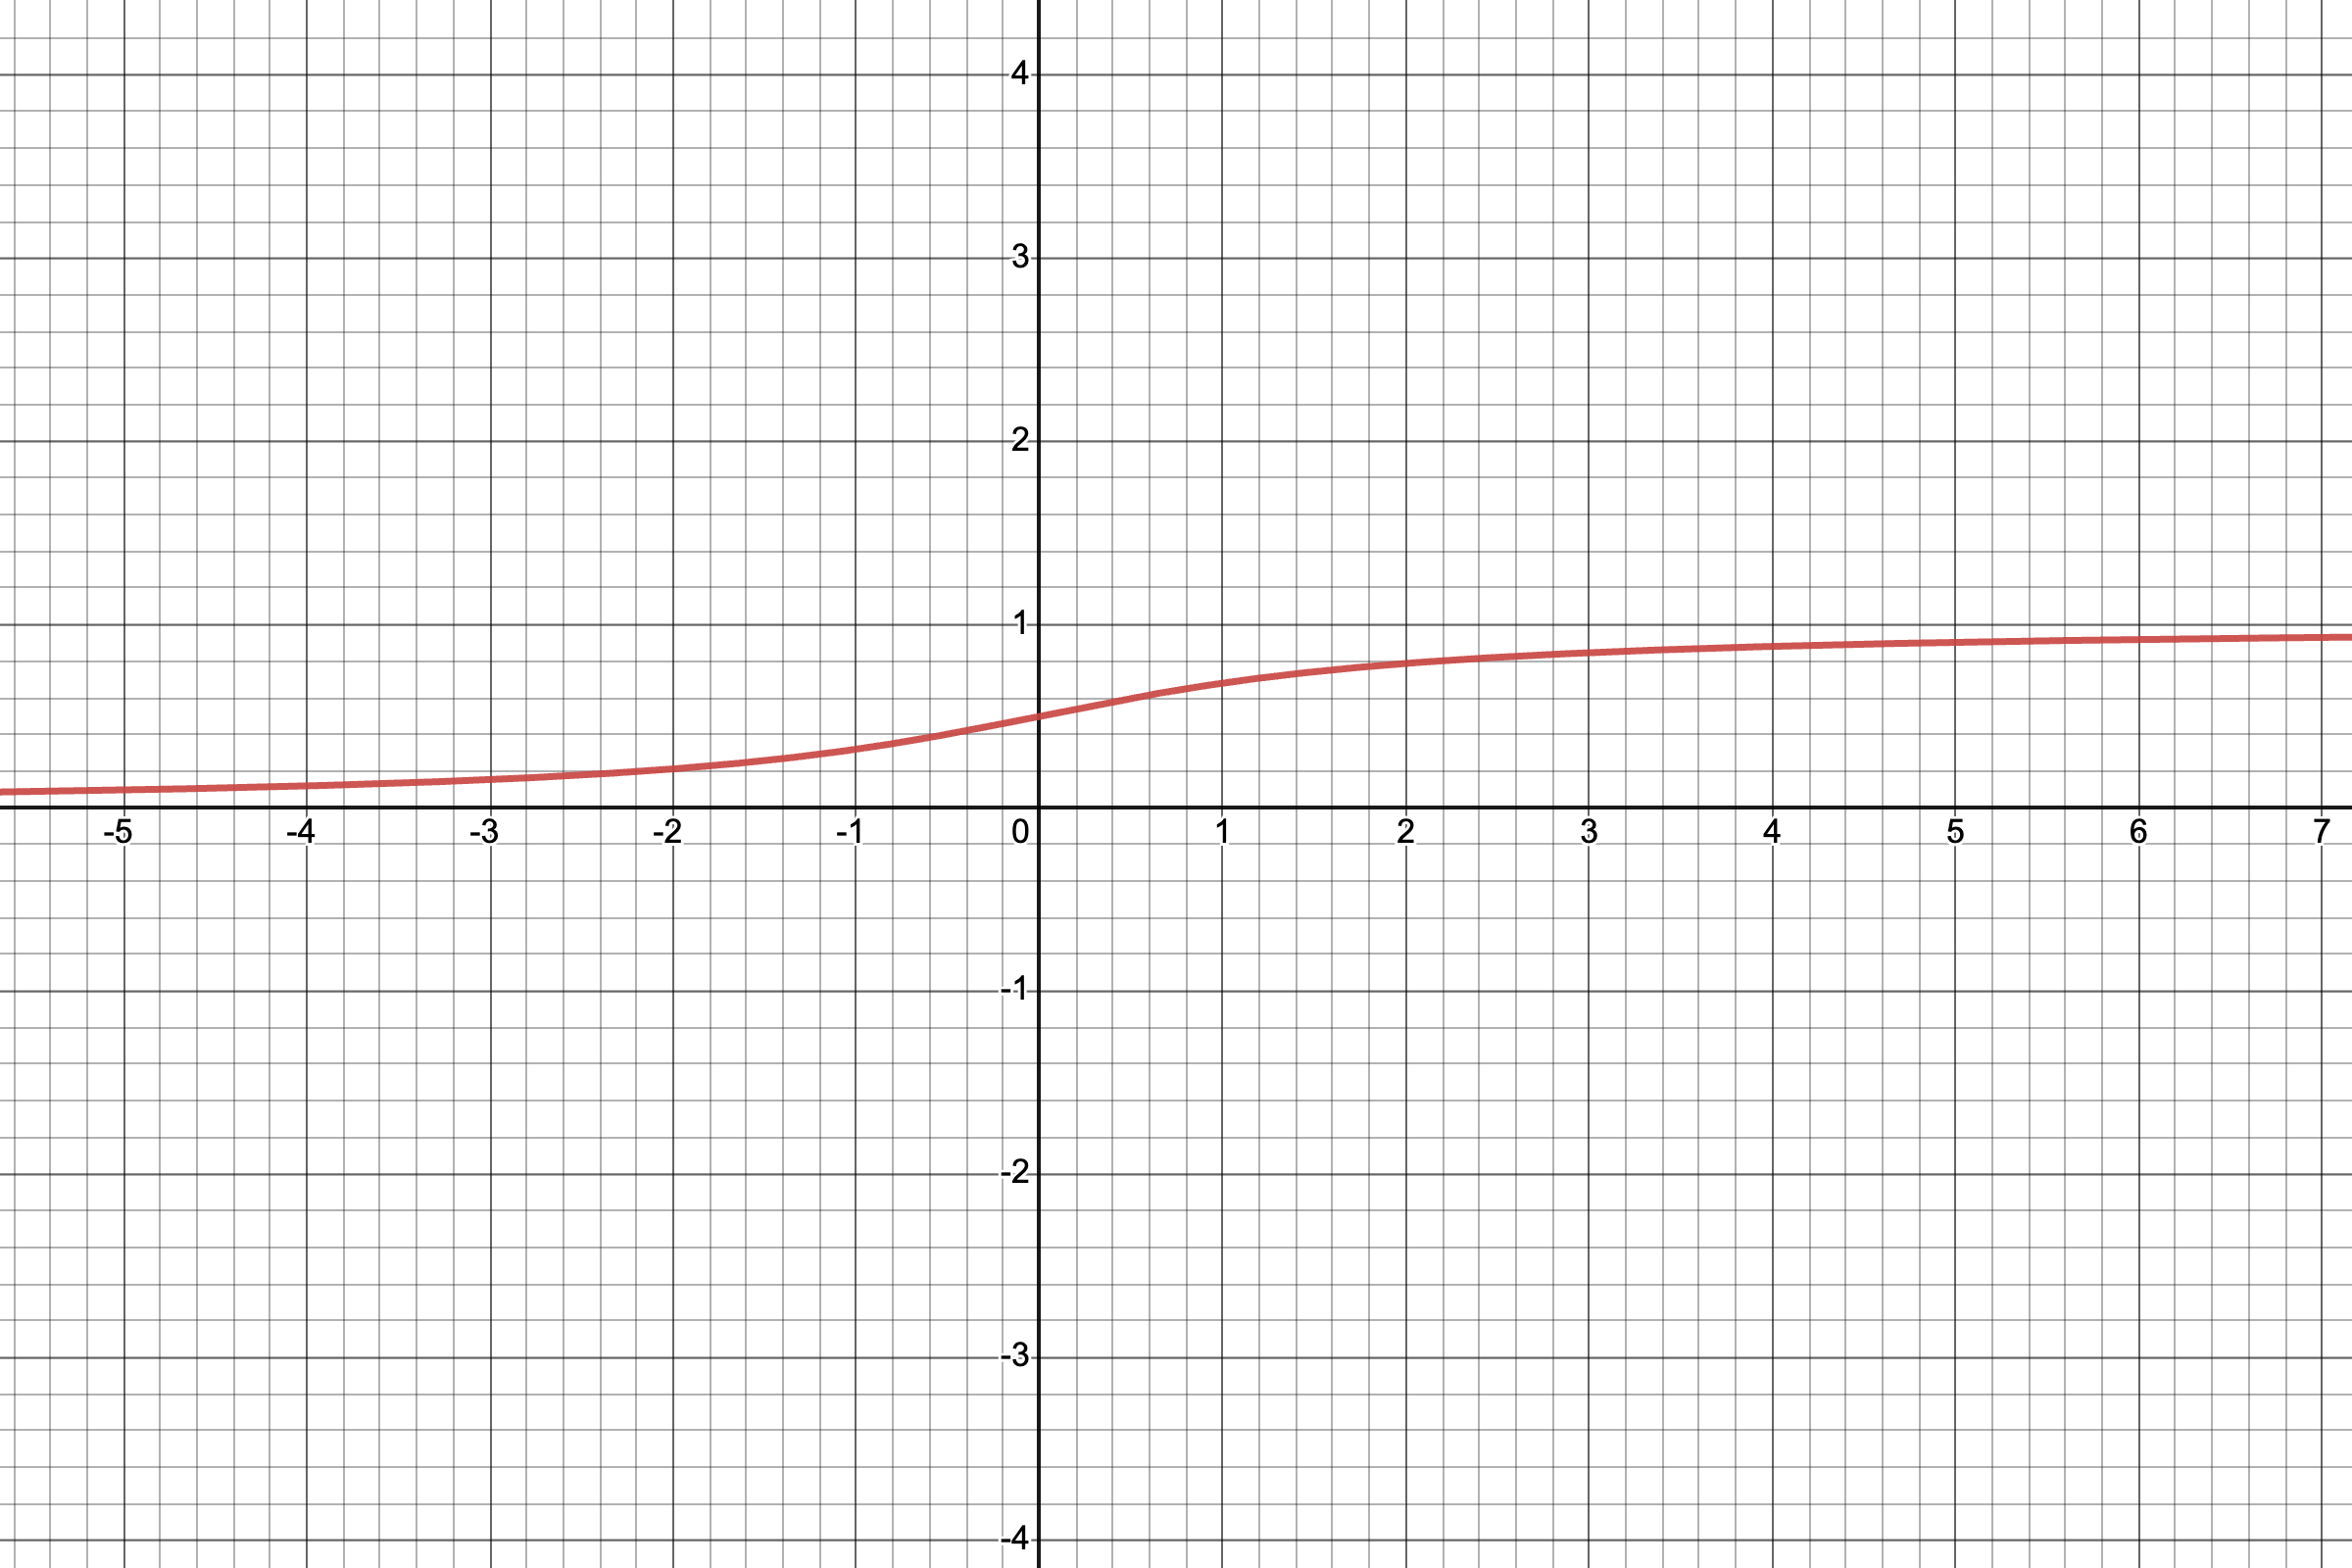
\includegraphics[width=0.7\linewidth]{hw2_figures/2.2b.png}
        \centering
        \caption{CDF $F_X(x)$}
    \end{figure}
\end{enumerate}
\hrule
\clearpage

\paragraph*{Problem 2.3} \hfill\\
\begin{align*}
    X\thicksim\mathcal{N}(5, 16)
\end{align*}
let us define $Y$ as $Y\triangleq\frac{X-5}{4}$, then
\begin{align*}
    Y\thicksim\mathcal{N}(0, 1)
\end{align*}
hence by using the change of variable ($X=4Y+5$) we will be able to calculate the probabilities based on the Q-function which is defined for the Standard Normal distribution ($\mathcal{N}(0, 1)$).
\begin{equation*}
    Q(y)=P[Y>y]=\int_y^\infty\frac{1}{\sqrt{2\pi}}\exp({-\frac{u^2}{2})du}
\end{equation*}
\begin{enumerate}[((a))]
    \item To calculate probabilities in this part we assumed that $Q(-x)=1-Q(x)$,which will be proved in section ((d)) of this problem.
    \begin{equation*}
        \mathbf{P[X>4]}=P[4Y+5>4]=P[Y>\frac{-1}{4}]=Q(\frac{-1}{4})=0.5987\\
    \end{equation*}
    Closed or open intervals for the Gaussian distributed random variable has no impact on the final probability value:
    \begin{equation*}
        \mathbf{P[X\geq7]}=P[4Y+5\geq7]=P[Y\geq\frac{1}{2}]=P[Y=\frac{1}{2}] + P[Y>\frac{1}{2}]=0+Q(\frac{1}{2})=0.3085
    \end{equation*}
    \begin{align*}
        \mathbf{P[2<X<7]}&=P[X>2]-P[X\geq7]=P[X>2]-P[X>7]\\
        &=P[4Y+5>2]-P[4Y+5>7]=P[Y>\frac{-3}{4}]-P[Y>\frac{2}{4}]\\
        &=Q(\frac{-3}{4})-Q(\frac{2}{4})=0.4648
    \end{align*}
    \begin{align*}
        \mathbf{P[6\leq X\leq8]}&=P[X\geq6]-P[X>8]=P[X>6]-P[X>8]\\
        &=P[4Y+5>6]-P[4Y+5>8]=P[Y>\frac{1}{4}]-P[Y>\frac{3}{4}]\\
        &=Q(\frac{1}{4})-Q(\frac{3}{4})=0.1747
    \end{align*}
    \item 
    \begin{align*}
        P[X<a]&=0.8869\\
        1-P[X>a]&=0.8869\\
        P[X>a]&=0.1131\\
        P[4Y+5>a]&=0.1131\\
        P[Y>\frac{a-5}{4}]&=0.1131\\
        Q(\frac{a-5}{4})&=0.1131 \qquad \text{(Q-function Table)}\\ 
        \frac{a-5}{4}&=1.2102\\
        a&=9.8408
    \end{align*}
    \item 
    \begin{align*}
        P[13<X\leq c]&=0.0123\\
        P[X>13]-P[X>c]&=0.0123\\
        P[4Y+5>13]-P[4Y+5>c]&=0.0123\\
        P[Y>2]-P[Y>\frac{c-5}{4}]&=0.0123\\
        Q(2)-Q(\frac{c-5}{4})&=0.0123 \qquad\qquad \text{(Q-function Table)}\\ 
        0.0228-Q(\frac{c-5}{4})&=0.0123\\
        \frac{c-5}{4}&=Q^{-1}(0.0105)\qquad \text{(Q-function Table)}\\
        c&=14.2391
    \end{align*}
    \item Before deriving the asked equation, we note that for a standard Gaussian random variable:
    \begin{align*}
        1&=\int_{-\infty}^{+\infty}\frac{1}{\sqrt{2\pi}}\exp({-\frac{u^2}{2})du}\\
        1&=\int_{-\infty}^x\frac{1}{\sqrt{2\pi}}\exp({-\frac{u^2}{2})du} + \int_x^\infty\frac{1}{\sqrt{2\pi}}\exp({-\frac{u^2}{2})du}\tag{$\dagger$}\\ 
        1&=\int_{-\infty}^x\frac{1}{\sqrt{2\pi}}\exp({-\frac{u^2}{2})du} + Q(x)
    \end{align*}
    Now we can derive $Q(-x)$:
    \begin{align*}
        Q(-x)&=\int_{-x}^\infty\frac{1}{\sqrt{2\pi}}\exp({-\frac{u^2}{2})du} \qquad \text{(change of variable: } v=-u)\\
        &=\int_{x}^{-\infty}\frac{-1}{\sqrt{2\pi}}\exp({-\frac{v^2}{2})dv}\\
        &=\int_{-\infty}^{x}\frac{1}{\sqrt{2\pi}}\exp({-\frac{v^2}{2})dv}\qquad (\text{using }(\dagger))\\
        &=1-\int_x^\infty\frac{1}{\sqrt{2\pi}}\exp({-\frac{u^2}{2})du}\\
        &=1-Q(x)
    \end{align*}
\end{enumerate}
\hrule
\clearpage
\paragraph*{Problem 2.4} \hfill\\
    \begin{enumerate}[((a))]
        \item Relative frequencies of $X$ and $Y$: 
        \begin{figure}[h!]
            \centering
            \subfigure[]{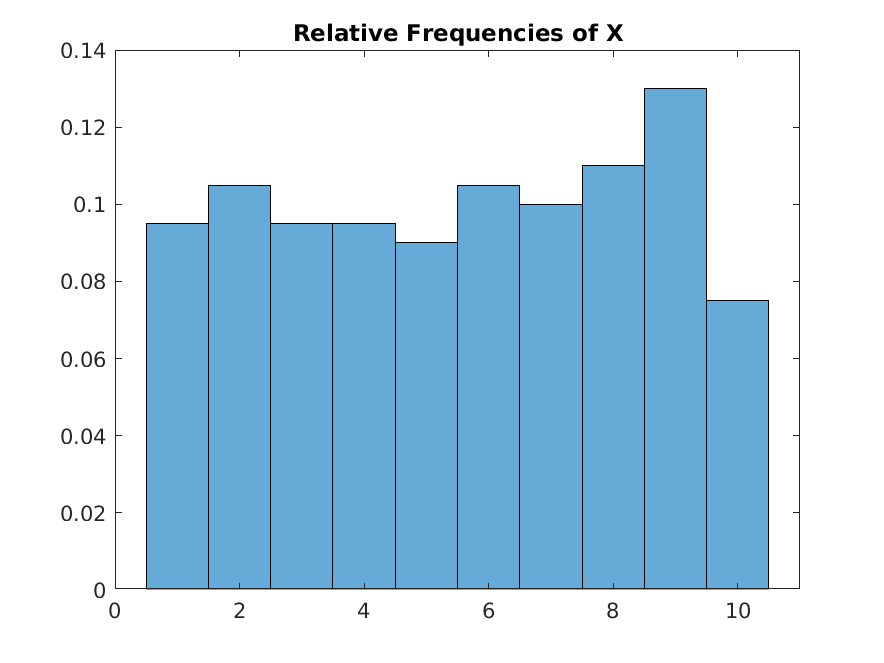
\includegraphics[width=0.49\textwidth]{hw2_figures/2.4a1.png}}
            \hfill
            \subfigure[]{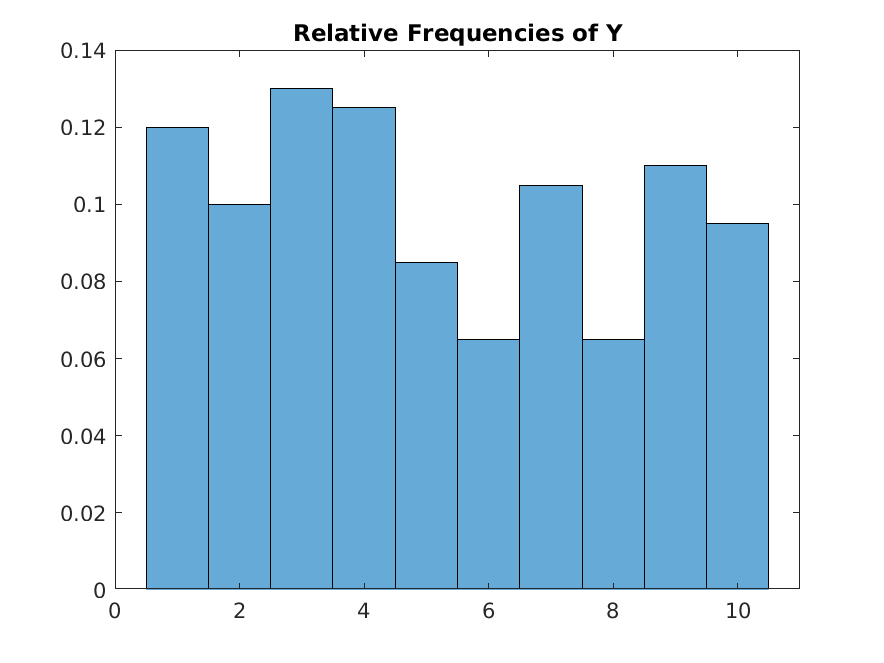
\includegraphics[width=0.49\textwidth]{hw2_figures/2.4a2.png}}
            \vfill
            \subfigure[]{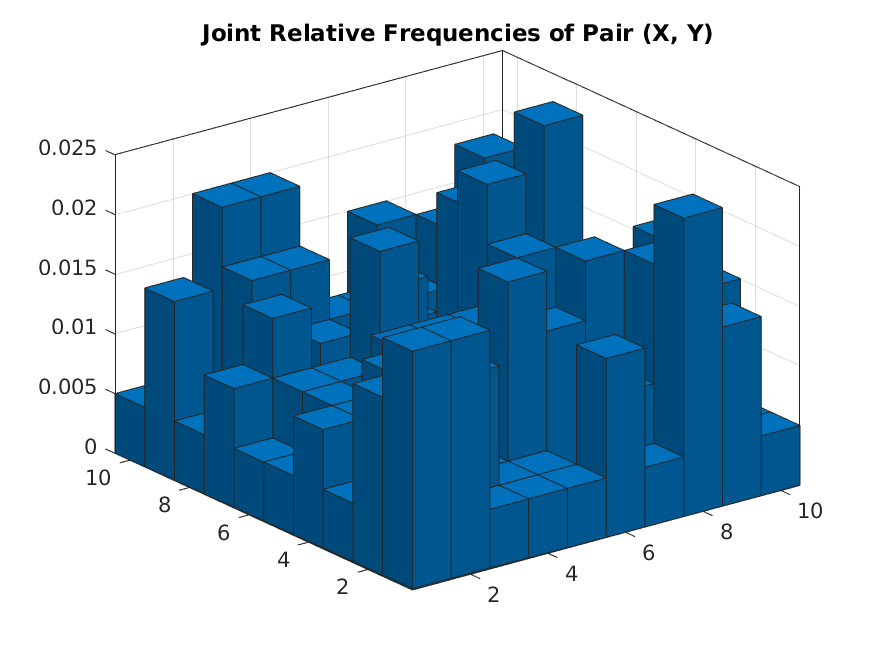
\includegraphics[width=0.5\textwidth]{hw2_figures/2.4a3.png}}
            \caption{200 pairs of $(X_i, Y_i)$ drawn uniformly from $\{1,2, \dots,10\}$.}
        \end{figure}
        \clearpage
        \item $Z$ which is sum of two uniform random variables, has a probability distribution which is the convolution of a uniform by itself. Therefore the distribution of $Z$ will have the shape of a Triangular function:
        \begin{figure}[h!]
            \centering
            \subfigure[]{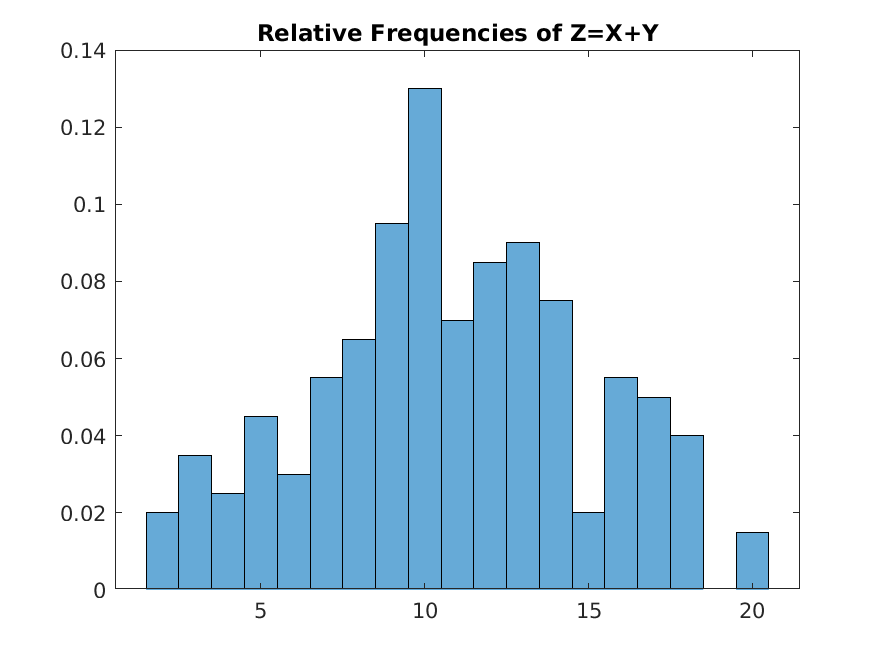
\includegraphics[width=0.7\textwidth]{hw2_figures/2.4b.png}}
            \caption{200 samples of $Z=X+Y$.}
        \end{figure}
        \clearpage
        \item Relative frequencies of $W=XY$. It looks like a Poisson distribution, $Pois(\lambda)$ with relatively small $\lambda$ :
        \begin{figure}[h!]
            \centering
            \subfigure[]{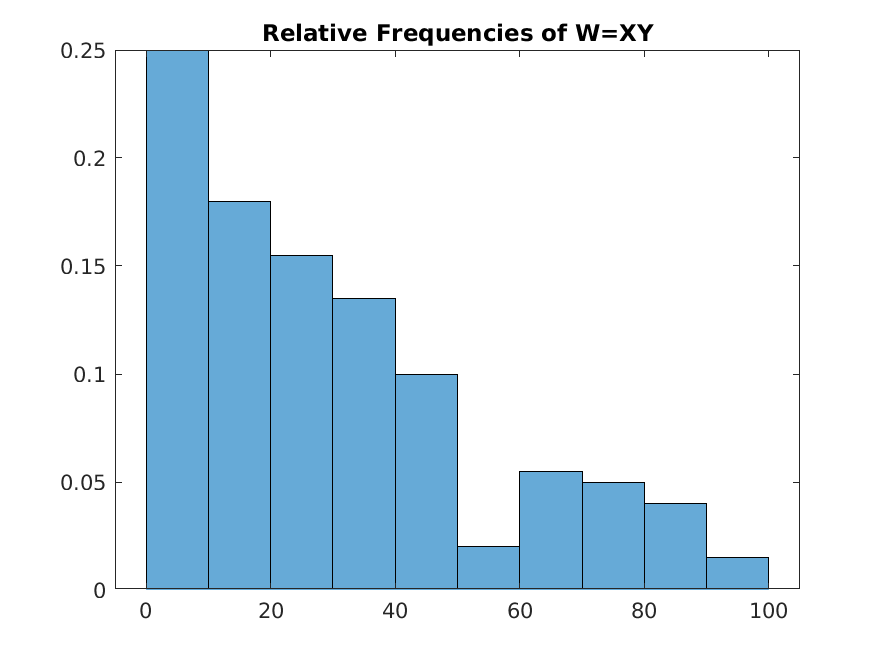
\includegraphics[width=0.7\textwidth]{hw2_figures/2.4c.png}}
            \caption{200 samples of $W=XY$.}
        \end{figure}
        \clearpage
        \item Relative frequencies of $V=X/Y$. It looks like a Poisson distribution, $Pois(\lambda)$ with relatively bigger $\lambda$:
        \begin{figure}[h!]
            \centering
            \subfigure[]{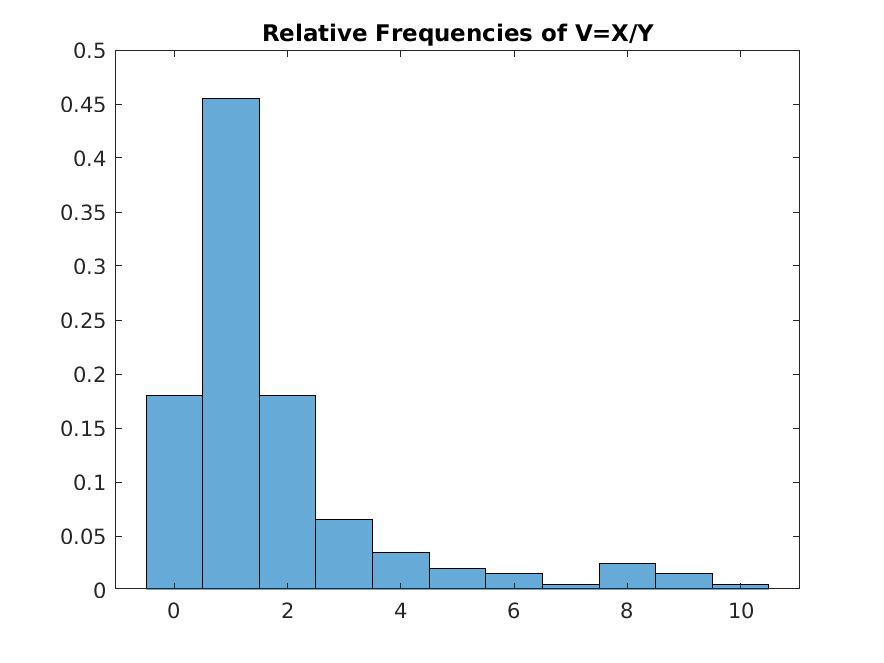
\includegraphics[width=0.7\textwidth]{hw2_figures/2.4d.png}}
            \caption{200 samples of $V=X/Y$.}
        \end{figure}
    \end{enumerate}
\hrule
\clearpage
\paragraph*{Problem 2.5} \hfill\\
    \begin{enumerate}[((a))]
        \item Relative frequencies of $X$ and $Y$: 
        \begin{figure}[h!]
            \centering
            \subfigure[]{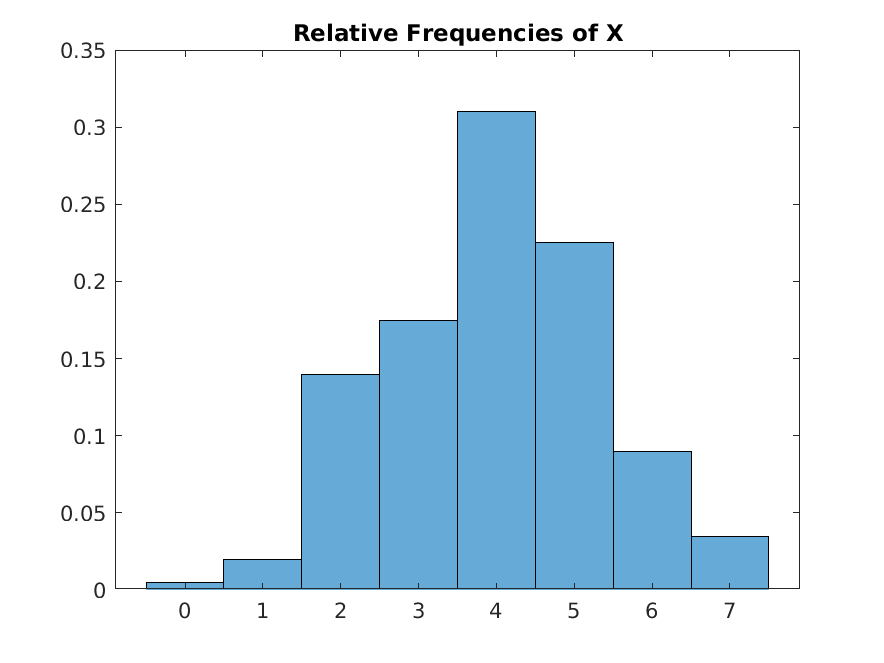
\includegraphics[width=0.49\textwidth]{hw2_figures/2.5a1.png}}
            \hfill
            \subfigure[]{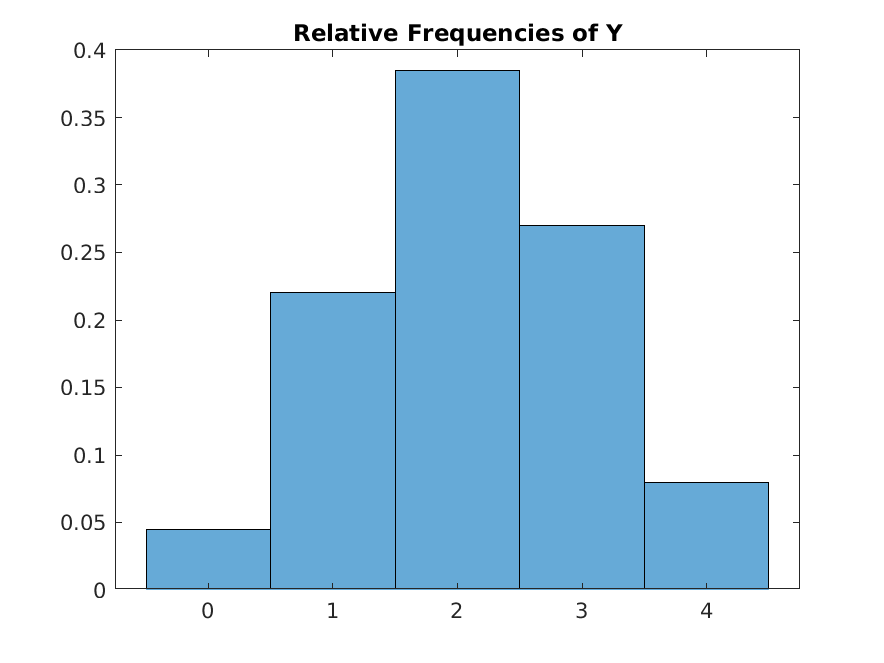
\includegraphics[width=0.49\textwidth]{hw2_figures/2.5a2.png}}
            \vfill
            \subfigure[]{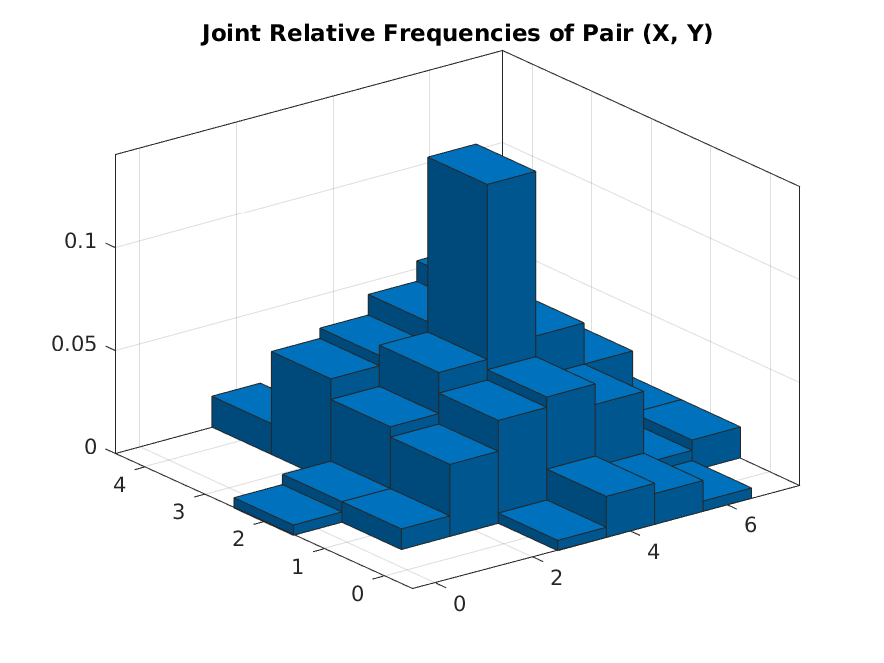
\includegraphics[width=0.5\textwidth]{hw2_figures/2.5a3.png}}
            \caption{200 pairs of $(X_i, Y_i)$ drawn from $Binomial(8, 0.5)$ and $Binomial(4, 0.5)$, respectively.}
        \end{figure}
        \clearpage
        \item Relative frequencies of $Z=X+Y$. Sum of these two binomial distributions will be also a binomial distribution with parameters $n=8+4$, $p=0.5$. The distribution with the expected value of 6 is discernible from the plot below:
        \begin{figure}[h!]
            \centering
            \subfigure[]{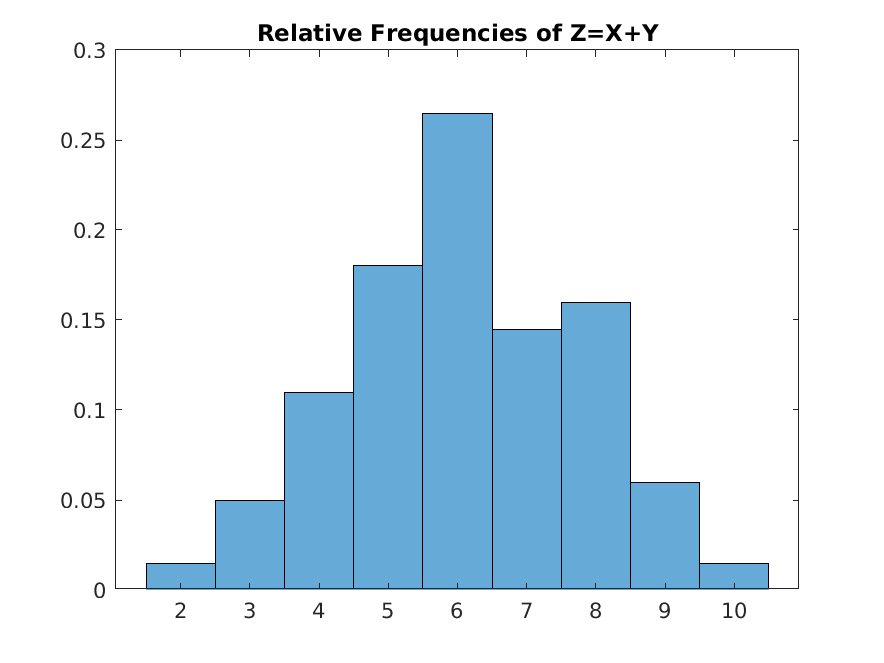
\includegraphics[width=0.7\textwidth]{hw2_figures/2.5b.png}}
            \caption{200 samples of $Z=X+Y$.}
        \end{figure}
    \end{enumerate}
\hrule
\clearpage
\paragraph*{Problem 2.6} \hfill\\
    \begin{enumerate}[((a))]
        \item Relative frequencies of $X$ and $Y$: 
        \begin{figure}[h!]
            \centering
            \subfigure[]{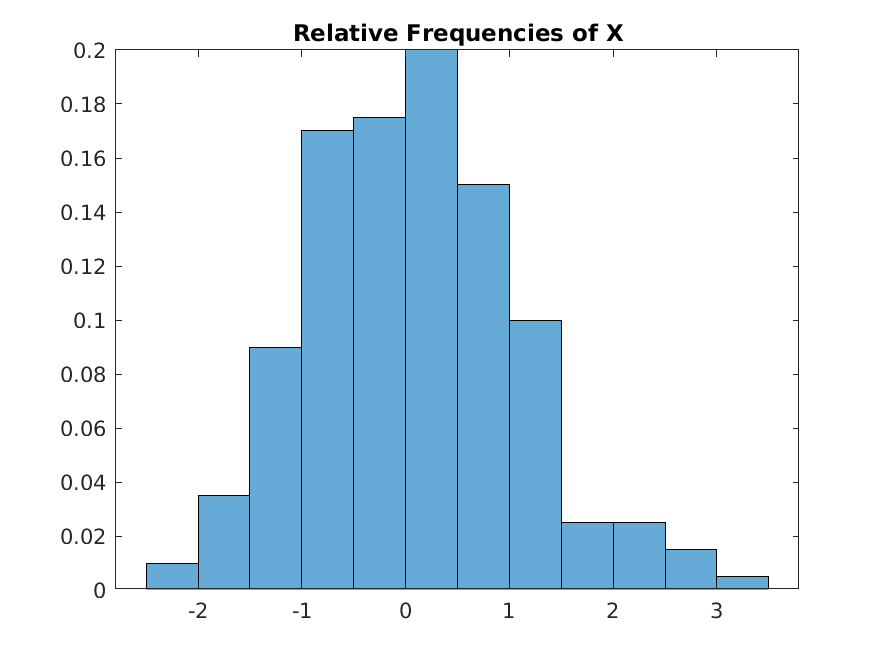
\includegraphics[width=0.49\textwidth]{hw2_figures/2.6a1.png}}
            \hfill
            \subfigure[]{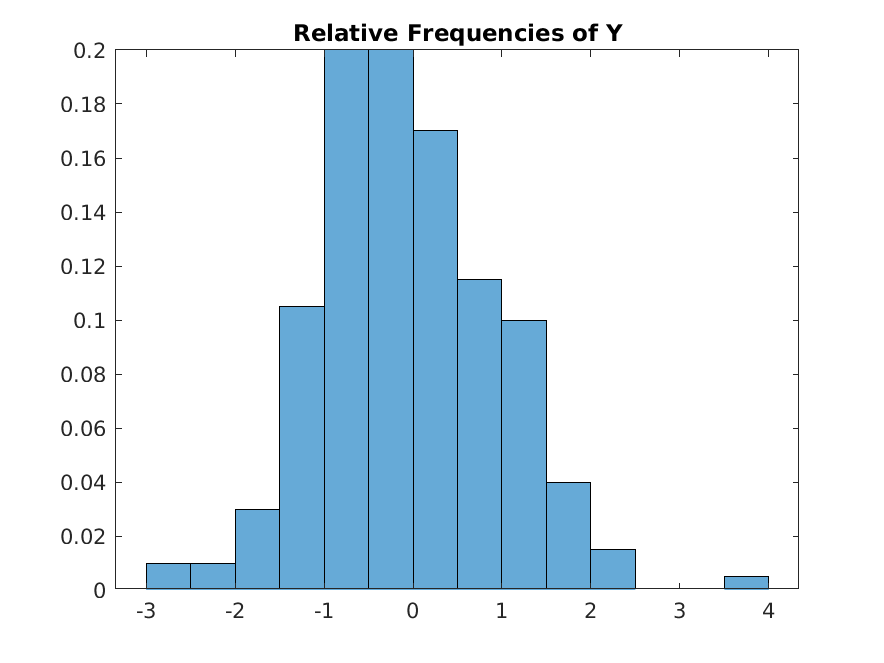
\includegraphics[width=0.49\textwidth]{hw2_figures/2.6a2.png}}
            \vfill
            \subfigure[]{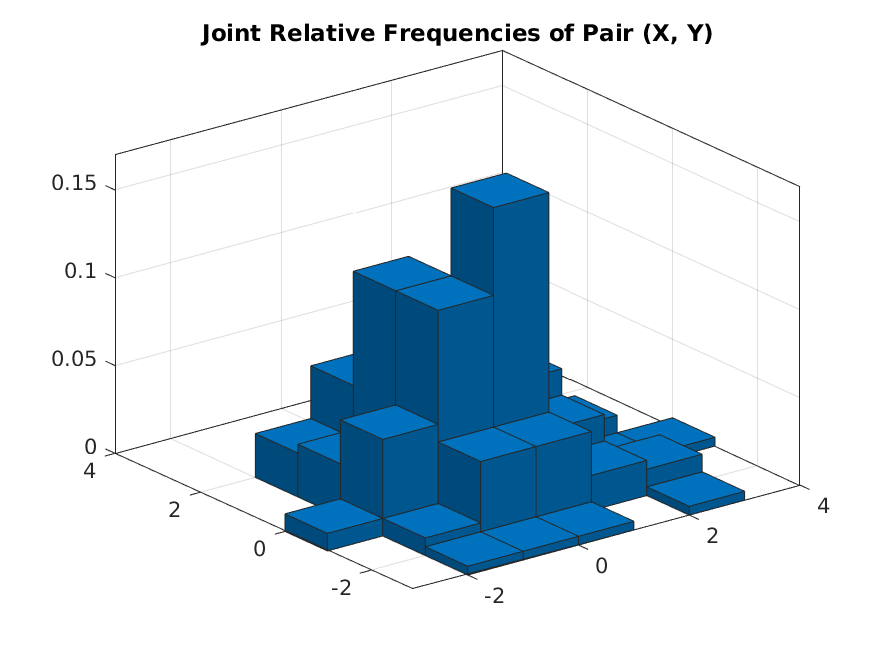
\includegraphics[width=0.5\textwidth]{hw2_figures/2.6a3.png}}
            \caption{200 pairs of $(X_i, Y_i)$ drawn from $\mathcal{N}(0, 1)$.}
        \end{figure}
        \clearpage
        \item Relative frequencies of $Z=X/Y$. The ratio of these two independent normally distributed random variable will follow Cauchy distribution as can be seen from the plot below:
        \begin{figure}[h!]
            \centering
            \subfigure[]{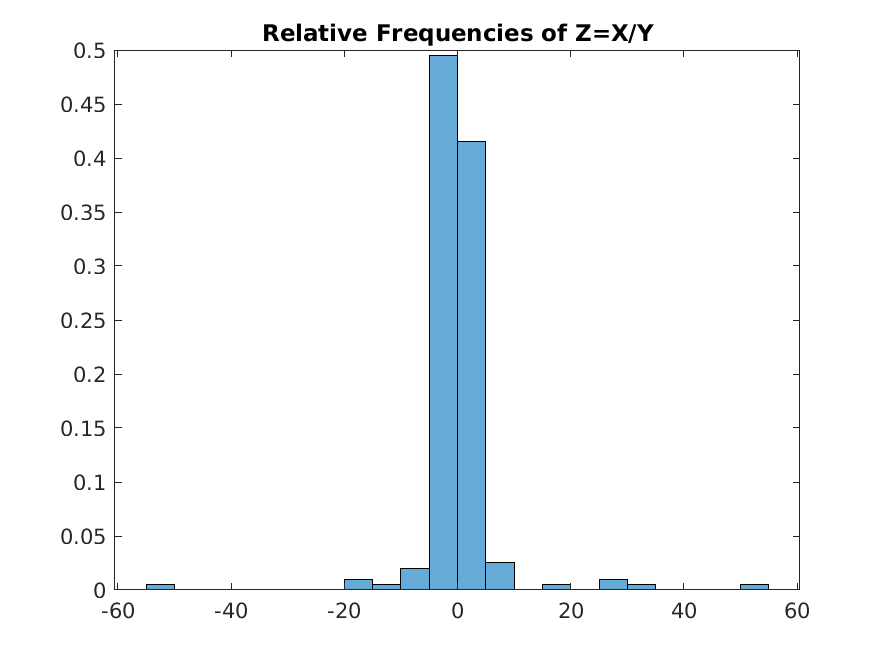
\includegraphics[width=0.7\textwidth]{hw2_figures/2.6b.png}}
            \caption{200 samples of $Z=X/Y$.}
        \end{figure}
        \clearpage
    \end{enumerate}
\hrule
\paragraph*{Problem 2.7} \hfill\\
    Relative frequencies of $Z=-ln(X)$, in which $X$ is drawn from $\mathcal{U}(0,1)$. The resulting $Z$ will follow an Exponential distribution, i.e. $Exp(\lambda)$, with parameter $\lambda=1$:
    \begin{figure}[h!]
        \centering
        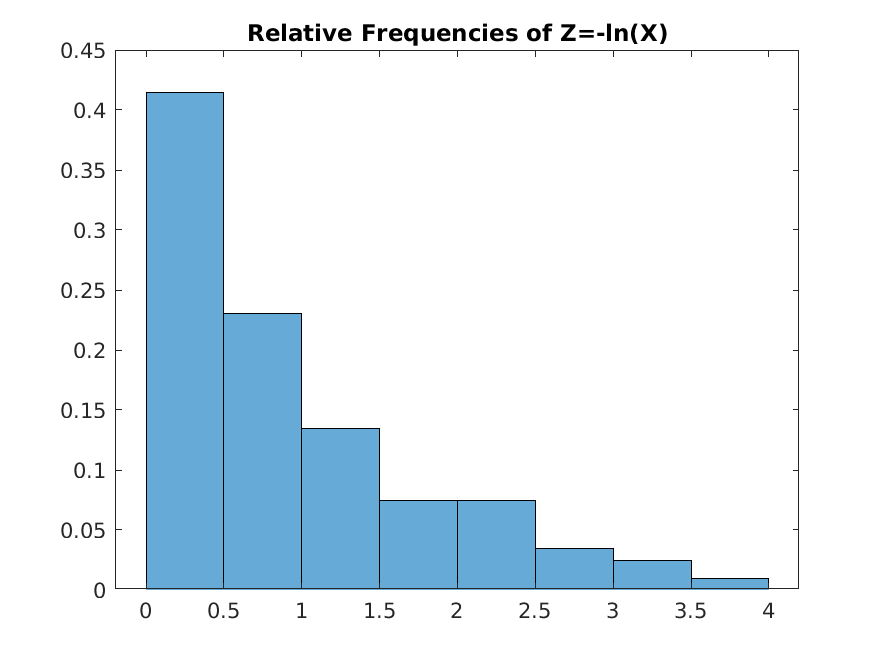
\includegraphics[width=0.7\textwidth]{hw2_figures/2.7.png}
        \caption{200 samples of $Z=-ln(X)$.}
    \end{figure}
    \clearpage
\hrule
\paragraph*{Problem 2.8} \hfill\\
\begin{enumerate}[((a))]
    \item The mean and variance of Binomial distribution:
    \begin{align*}
        E(X)&=n.p=8\times0.5=4\\
        Var(X)&=n.p.(1-p)=8\times0.5\times0.5=2
    \end{align*}
    \item
    \begin{align*}
        M_{200}&=3.9750 \qquad\Rightarrow\qquad |Error_{mean}|=0.025\\
        V_{200}&=1.9039 \qquad\Rightarrow\qquad |Error_{var}|=0.0961
    \end{align*}
    \begin{figure}[h!]
        \centering
        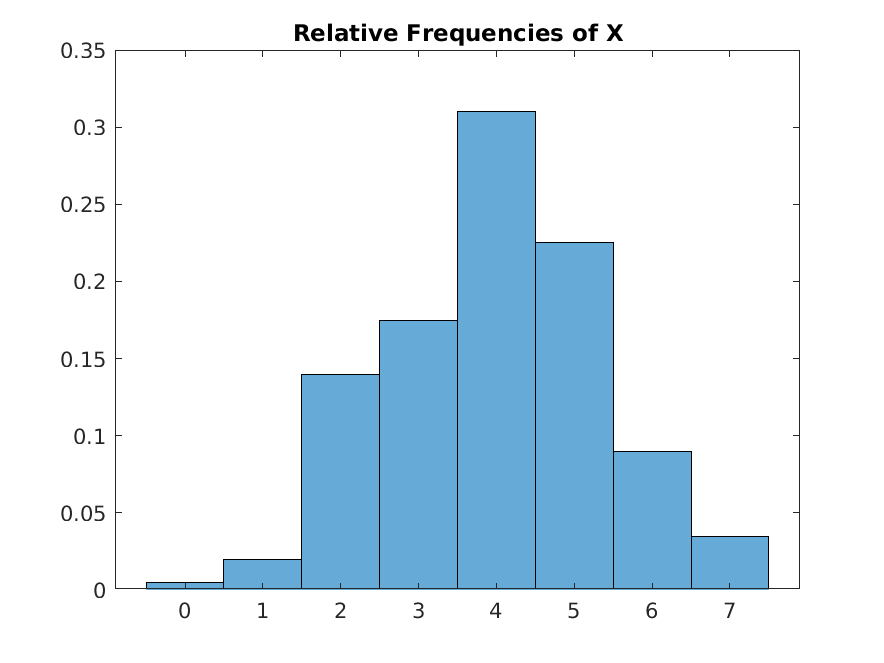
\includegraphics[width=0.7\textwidth]{hw2_figures/2.8.png}
        \caption{200 samples of $X$.}
    \end{figure}
    \clearpage
\end{enumerate}
\hrule
\paragraph*{Problem 2.9} \hfill\\
\begin{enumerate}[((a))]
    \item The mean and variance of $Y$:
    \begin{align*}
        E(Y)&=E(2X+5)=2E(X)+5=5\\
        Var(Y)&=Var(2X+5)=4Var(X)=4
    \end{align*}
    \item
    \begin{align*}
        M_{200}&=5.1483 \qquad\Rightarrow\qquad |Error_{mean}|=0.1483\\
        V_{200}&=3.9714 \qquad\Rightarrow\qquad |Error_{var}|=0.0286
    \end{align*}
    Relative frequencies of $Y=2X+5$:
    \begin{figure}[h!]
        \centering
        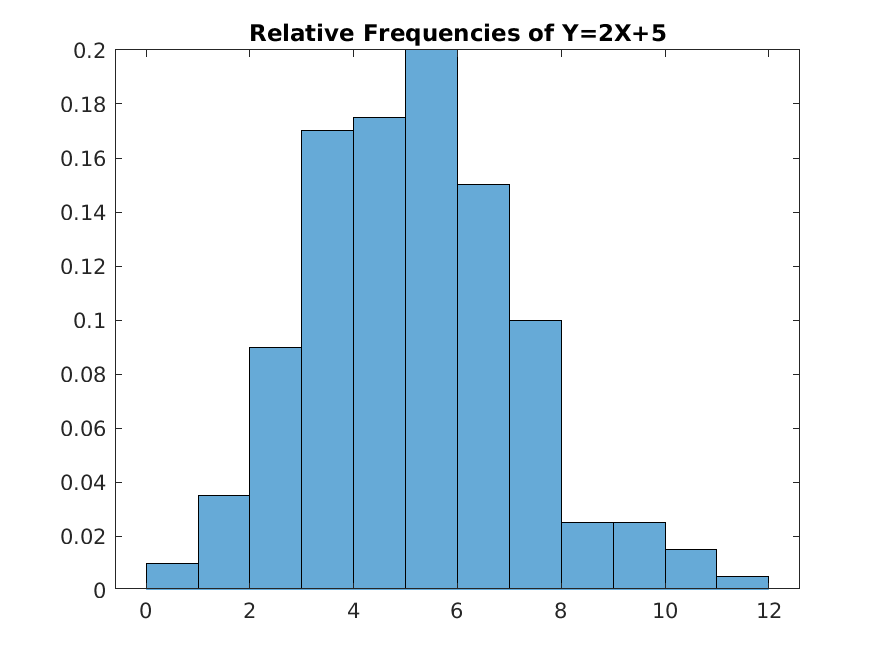
\includegraphics[width=0.7\textwidth]{hw2_figures/2.9.png}
        \caption{200 samples of $Y=2X+5$.}
    \end{figure}
\end{enumerate}
\hrule
\end{document}

